\section{Maximum Likelihood Estimation}

In the current section,
the parameters \(\beta, \gamma, t^*\) will be considered to be distributed, according to some known distribution.
This makes the outcomes of the function \(t^{opt}(\beta, \gamma, t^*)\) defined above to be distributed themselves,
according to a distribution that can be explicitly characterized,
by finding an expression for its probability density function.

Once the probability density function has been found,
its evaluation can yield an expression for the likelihood of a given dataset of arrival times.
This allows the estimation of parameters that have an influence on the original distribution,
by doing a Maximum Likelihood Estimation.

\subsection{Theoretical Prerequisites}


The goal of the section is thus to find an analytical expression for the Probability Density Function that characterizes the distribution of the outcomes of the function \(t^{opt}\).
To this end, the characterization developed in the preceding section will be employed,
in a slightly simpler setting, in which some additional hypotheses on the travel time function are made.

The assumptions that simplify the estimation are shown in the following definition:
\begin{definition}
  \label{def:proper_tt}
  Let \(tt_a:\R\rightarrow\R\).

  \(tt_a\) is a \textbf{Proper Travel Time Function} if \(tt_a\) is a General Travel Time Function and,
  on top of this, 
  there exist two time points \(k_1 \neq k_2 \in \R\) such that,
  in the subsets
  \begin{align}
    \label{eq:subs_conc_conv}
    \mathcal{D}_{conc} = (k_1, k_2) && \mathcal{D}_{conv} = \R \setminus \mathcal{D}_{conc}
  \end{align}
  The function \(tt_a\) satisfies the following:
  \begin{enumerate}
  \item \(tt_a\) is concave on the domain \(\mathcal{D}_{conc}\)
  \item \(tt_a\) is convex on the domain \(\mathcal{D}_{conv}\)
  \end{enumerate}
\end{definition}
\todo{Why is proper tt even realistic?}

\begin{figure}
  \centering
  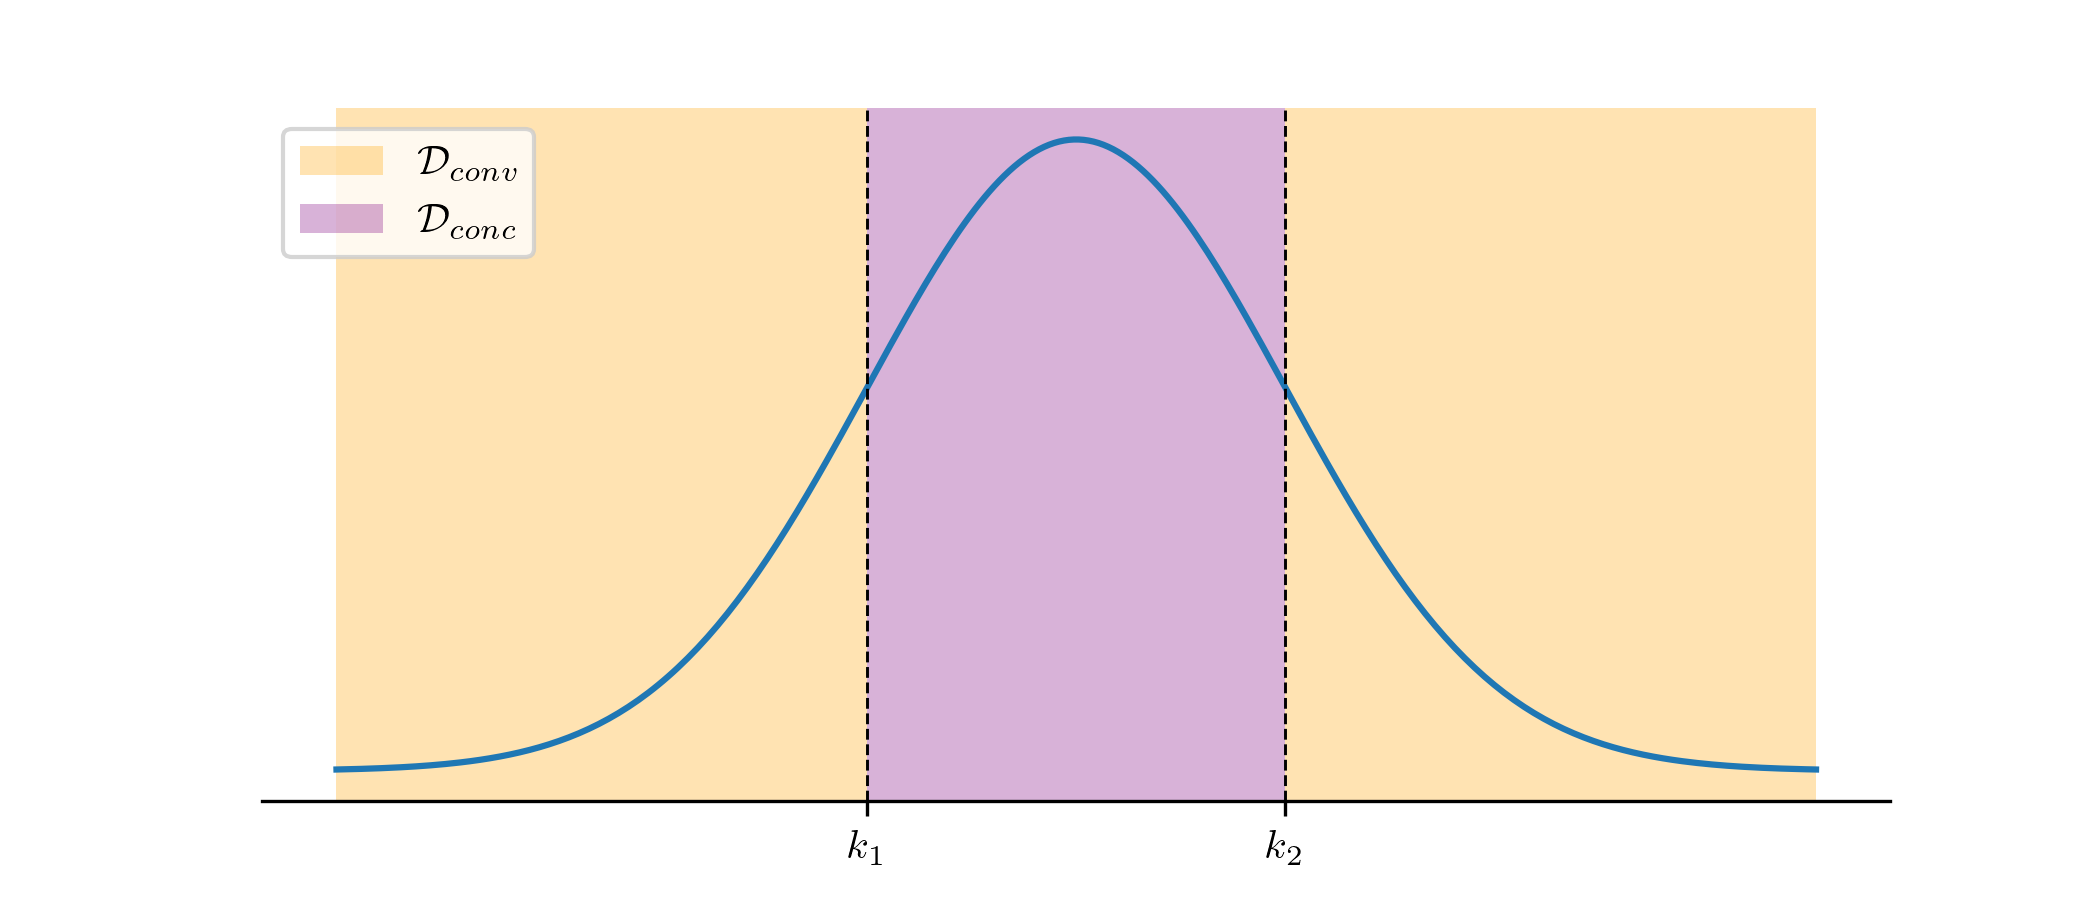
\includegraphics[width=.9\textwidth]{conv_conc_gauss}
  \caption{
    Example of a proper travel time function.
  The shaded zones show the parts of its domain in which the function is convex or concave.}
  \label{fig:conc-conv-gauss}
\end{figure}

An example of such a function is the gaussian function,
shown in Figure~\ref{fig:conc-conv-gauss} with the corresponding subsets \(\mathcal{D}_{conc}, \mathcal{D}_{conv}\).

For a proper travel time function,
the estimation of the optimal arrival time \(t^{opt}\) considerably simplifies:
the following observation shows how.
\begin{obs}
  \label{obs:simplified-char}
  Consider the problem of choosing an optimal departure time
  with a proper travel time function, and let \(\beta, \gamma\) be fixed.

  There exist two intervals \((t_i^e, t_f^e), (t_i^l, t_f^l)\) such that an on-time arrival \(t^{opt} = t^*\) is realized if and only if
  \begin{equation*}
    t^* \notin (t_i^e, t_f^e) \cup  (t_i^l, t_f^l)
  \end{equation*}
\end{obs}

Note that this is implied from what said by Proposition~\ref{prop:into-early-late},
except for a single detail:
the intervals are indeed here at most one (for each type of arrival), rather than an arbitrary number.

This is a consequence of the hypothesis on the travel time function:
the point \(t_i^e\) must indeed be an eligible early arrival and,
as shown in Lemma~\ref{lemma:bounded-der-tt} and~\ref{lemma:cost_decoupled},
any possible early arrival must satisfy two simple conditions:
\begin{enumerate}
\item \(tt_a'(t_i^e) = \beta\)
\item \(tt_a''(t_i^e) \geq 0\)
\end{enumerate}
where the second one derives from being a minimum:
if the second derivative was negative, the point was indeed a maximum.

\begin{figure}
  \centering
  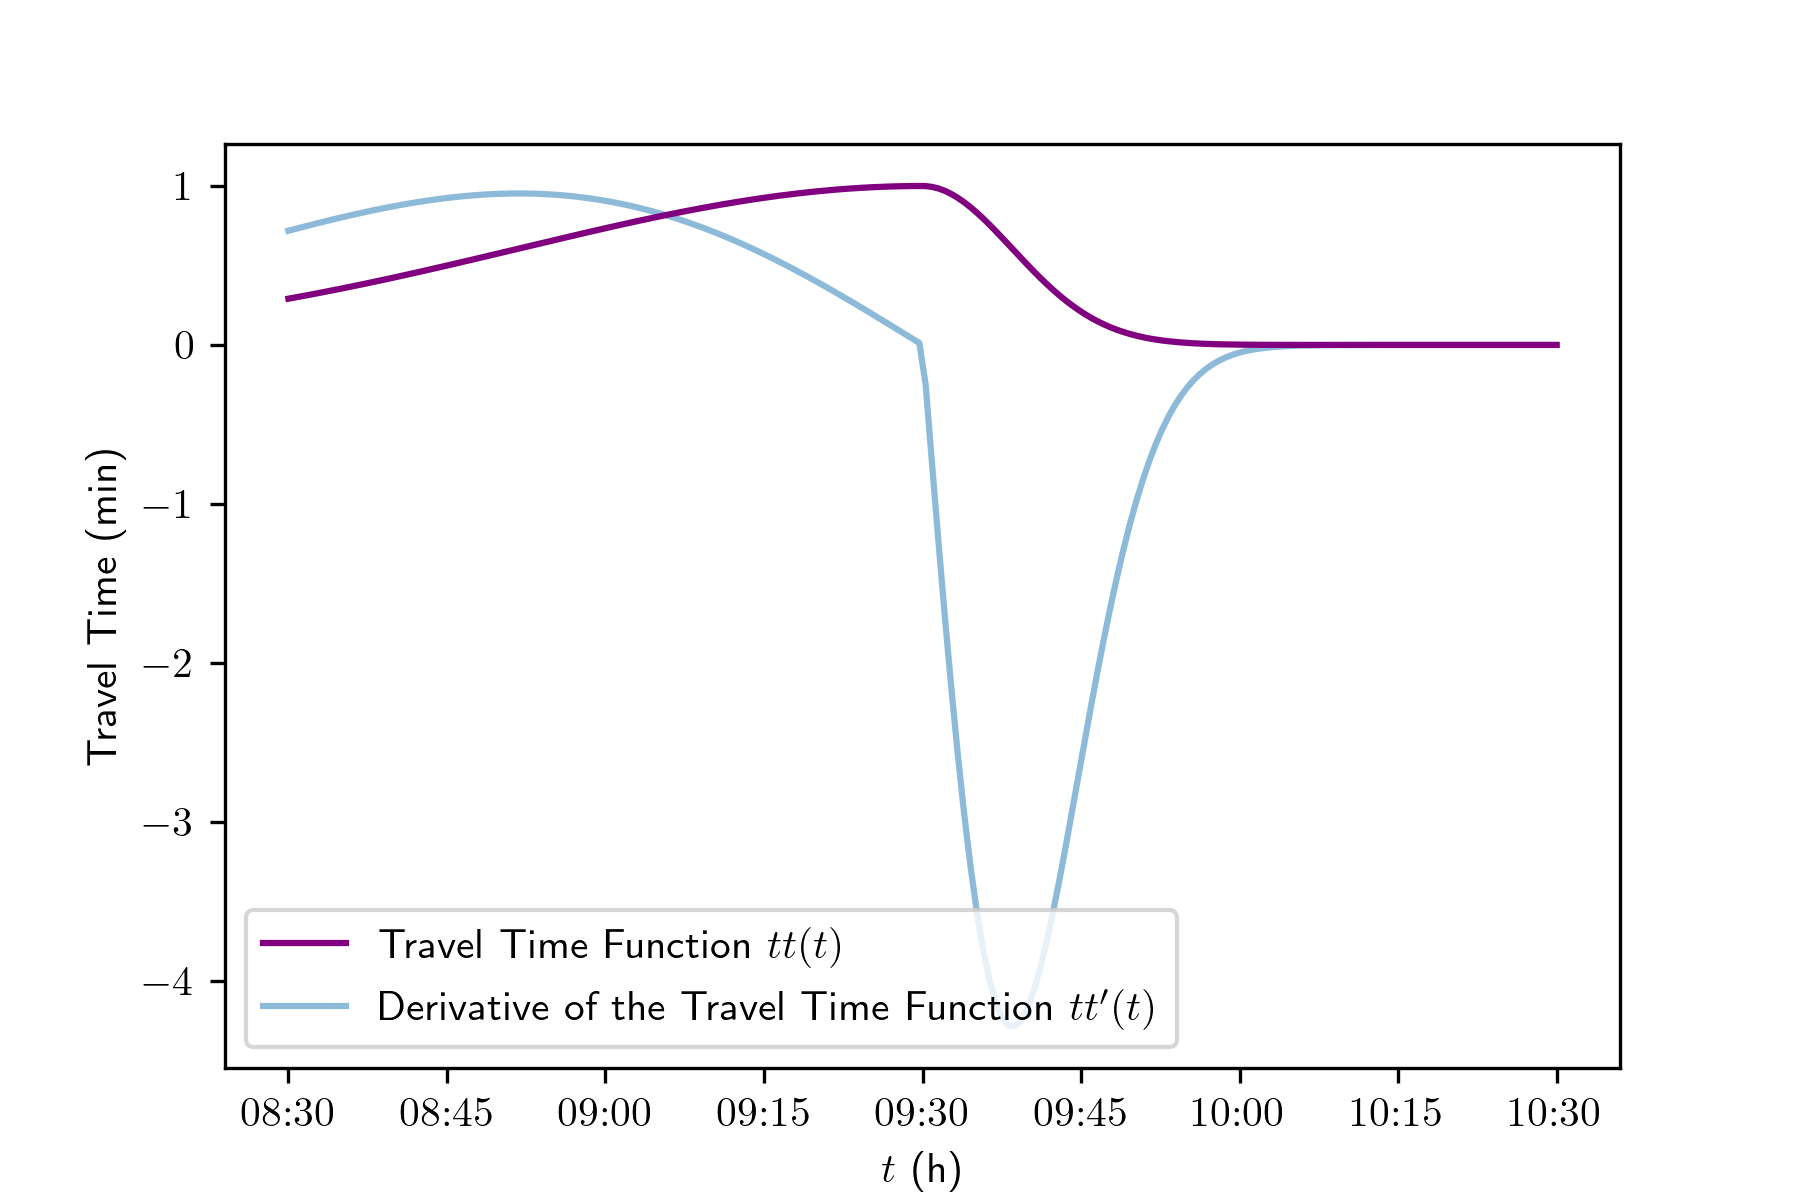
\includegraphics[width=.5\textwidth]{theo_tt}
  \caption{
    Example of a proper travel time function \(tt_a(t)\),
  plotted with its derivative.}
  \label{fig:theo_tt}
\end{figure}

But for a proper travel time function,
a point satisfying the conditions above can occur only once:
given the unimodality,
the function will be as shown in Figure~\ref{fig:theo_tt}: increasing, with an increasing derivative,
for \(t < k_1\), and decreasing with an increasing derivative for \(t > k_2\).
Its derivative will thus be injective on the convex part \(\mathcal{D}_{conv}\),
that is the only part in which the second derivative is non-negative.

Being the derivative injective,
there is at most one point \(t_i^e\) satisfying the condition \(tt_a(t_i^e) = \beta\).
The set \(E\) is thus either empty or a singleton.
A similar reasoning holds for late arrivals.

Consider thus now the problem of finding the intervals \((t_e, \bar{t_e})\), \((\bar{t_l}, t_l)\).
The points in which the arrivals occur are now easy to estimate. Let
\begin{equation*}
  \beta_{max} = \max_t tt_a'(t)\qquad \gamma_{max} = -\min_t tt_a'(t)
\end{equation*}

The following functions are well defined:
\begin{align*}
  t_i^e: (0, \beta_{max}) & \rightarrow \mathcal{D}_{conv}  & t_e^l: (0, \gamma_{max}) & \rightarrow \mathcal{D}_{conv} \\
       \beta & \mapsto (tt_a' |_{\mathcal{D}_{conv}})^{-1}(\beta) & \gamma & \mapsto(tt_a' |_{\mathcal{D}_{conv}})^{-1}(\gamma)
\end{align*}

\begin{figure}
  \centering
  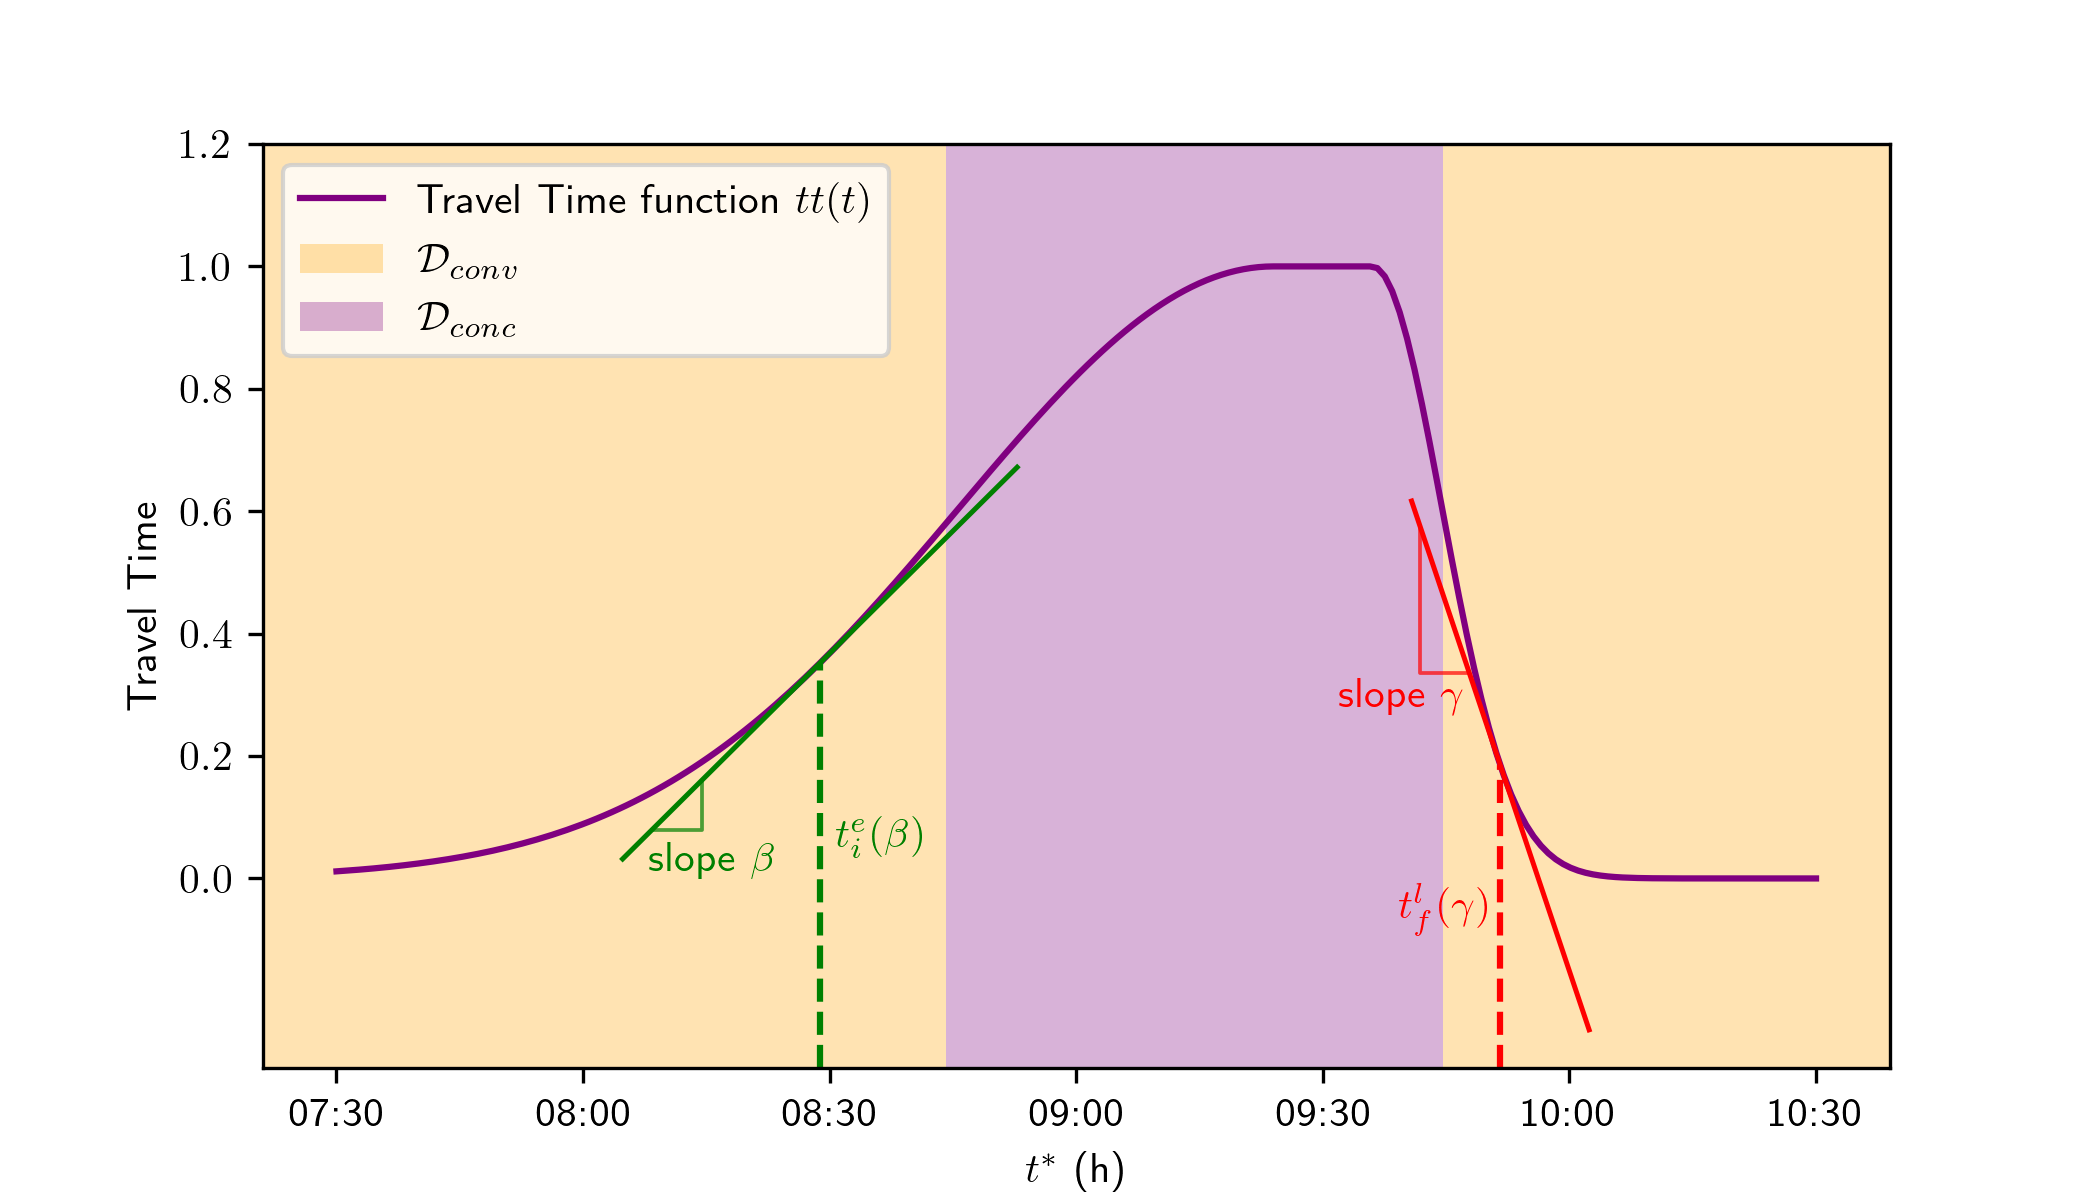
\includegraphics[width=.9\textwidth]{tang_cond}
  \caption{
    Proper travel time function,
    in which the results of the functions \(t_i^e(\beta), t_f^l(\gamma)\) are shown.
    The highlighted zones show the domains \(\mathcal{D}_{conc}, \mathcal{D}_{conv}\),
    that restrict the zones in which the derivative is inverted.
}
  \label{fig:tang-cond}
\end{figure}

Figure~\ref{fig:tang-cond} shows the outcomes of these functions on a theoretical proper travel time function

The functions \(t_i^e, t_f^l\) compute thus the initial point of the interval that yields early arrivals,
as well as the final point of the interval that yields late arrivals.

Estimating the remaining points \(t_f^e, t_i^l\) is slightly more difficult.
The expression in the proof of Proposition~\ref{prop:into-early-late} can anyway be used:
the function \(t_f^e(\beta), t_i^l(\gamma)\)
are thus defined as the points in which the line tangent to the travel time function at the initial points
(that are, the solid lines in Figure~\ref{fig:tang-cond})
intersect a second time with the travel time function.


A graphical representation of the functions \(b_i, b_e, g_i, g_e\) is shown in figure\todo{ref}
\todo{Here, how \(t_s\) is computed has to be explained. These things are to be put in this or in the theory section?? Maybe theory}
Once these functions have been defined,
the probability density function that characterizes the distribution of the optimal departure time \(t^{opt}\) can be computed.

\subsection{The Probability Density Function}

Consider now the same problem in which,
instead of the parameters \(\beta, \gamma, t^*\),
we consider three random variables \(B, \Gamma, T^*\).

A random variable for the optimal arrival will be defined as follows:
\begin{equation}
  \label{eq:rv-opt-arr}
  T^{opt} = t^{opt}(B, \Gamma, T^*)
\end{equation}

The goal of this section will be finding the density \(f_{T^{opt}}\) of the variable \(T^{opt}\).

In order to simplify the estimation process, an assumption (which is, indeed, quite restrictive)
is made on these random variable:

\begin{assumption}
  The random variables \(B, \Gamma, T^*\) are pairwise independent
\end{assumption}

Note that this assumption is rather significant,
but not as significant as it may sound:
remind indeed that, being the parameter \(\alpha\) in equation~\eqref{eq:cost_ta} normalized to 1,
the parameters \(\beta, \gamma\) represent the normalized values of the early and late arrival penalties instead of the actual ones,
and the assumption of independence is thus more realistic than how it was if the parameters were not normalized.

In the first place,
 it is convenient to distinguish between early, late and on-time arrivals.
In order to make this distinction, we define another random variable:
\begin{definition}
  Consider the function
  \begin{equation*}
    q(\beta, \gamma, t^*) =
    \begin{cases}
      -1 & \text{if } t^{opt}(\beta, \gamma, t^*) = t_e^{opt}(\beta, \gamma, t^*) \\
      0 & \text{if } t^{opt}(\beta, \gamma, t^*) = t^* \\
      1 & \text{if } t^{opt}(\beta, \gamma, t^*) = t_l^{opt}(\beta, \gamma, t^*)
    \end{cases}
  \end{equation*}

  Given the random variables \(B, \Gamma, T^*\), the random variable \(Q\) is defined as follows:
  \begin{equation*}
    Q  = q(B, \Gamma, T^*)
  \end{equation*}
\end{definition}

In practical terms, the random variable \(Q\) shows whether an early, on-time or late arrival is realized,
and takes the value \(-1\) if the optimal arrival is an early arrival,
\(1\) if it is a late arrival and \(0\) if it is an on-time one.

Since an optimal arrival can only be early, on-time or late,
by using the sum rule,
the probability density function for the random variable \(T^{opt}\) can be decomposed into three different parts:
\begin{equation}
  \label{eq:pdf-decomposed-q}
  f_{T^{opt}}(t) = f_{T^{opt}, Q}(t, -1) + f_{T^{opt}, Q}(t, 0) + f_{T^{opt}, Q}(t, 1)
\end{equation}
\todo{Where \(f_{T^{opt}, Q}\) is...}
The single addends are easier to describe,
and will be individually studied in the following.

\subsubsection{On-time Arrivals}

The value of the function
\begin{equation*}
  f_{T^{opt}, Q}(t, 0)
\end{equation*}
will be here computed.
This represents how likely is a value for the arrival time \(t\) to be an on-time arrival.

Note that Observation~\ref{obs:simplified-char} fully characterizes the values of the parameters for which the on-time arrivals are realized:
we are able, by using this characterization, to better describe the event at issue.

In particular, we note that the arrival time \(t\) is an optimal on-time arrival if and only if two conditions are satisfied at the same time:
the time \(t\) has to be a realization of the desired arrival time \(T^*\),
and it has to  be out from the intervals \((b_i(B), b_e(B)), (g_i(\Gamma), g_e(\Gamma))\).

Being the random variable \(T^*\) independent from \(B, \Gamma\),
the two events above are independent and their likelihood can be multiplied:
\begin{equation}
  \label{eq:on-time-intro}
  f_{T^{opt}, Q}(t, 0) = f_{T^*}(t) \cdot \prob(t \notin (b_i(B), b_e(B)) \cup (g_i(\Gamma), g_e(\Gamma)))
\end{equation}
where \(f_{T^*}\) is the probability density function of the random variable \(T^*\), and is known.

Expression~\eqref{eq:on-time-intro} leads to a straightforward way of computing the desired value:
the probability of being out from the intervals \((b_i(B), b_e(B)), (g_i(\Gamma), g_e(\Gamma))\) can indeed be simply evaluated by integration:

\begin{equation}
  \label{eq:prob-not-intervals}
  \prob( t \not\in (b_i(B), b_e(B)) \cup (g_i(\Gamma), g_e(\Gamma))) = \int_{b\in \R \vert t \not\in (b_i(b), b_e(b))}\int_{g \in \R \vert t \not\in (g_i(g), g_e(g))}f_B(b)f_\Gamma(g)\, dg\, db
\end{equation}
where \(f_B, f_\Gamma\) are the probability densities of, respectively, the random variables \(B, \Gamma\).


It is now possible to take advantage of Proposition\todo{Need to add this proposition somewhere...}:
the monotonicity of the intervals imply that there exist two functions representing the maximum values that \(\beta\) and \(\gamma\) can assume while keeping a given point into the defined intervals:
\begin{equation}
  \label{eq:def_b_0_g_0}
  \begin{split}
    \beta_0:\R&\rightarrow(0, \beta_{max}) \\
    t&\mapsto \sup\{b | t \in (b_i(b), b_e(b))\} \\[1em]
    \gamma_0:\R&\rightarrow(0, \gamma_{max}) \\
    t&\mapsto \sup\{g | t \in (g_i(g), g_e(g))\}
  \end{split}
\end{equation}

The definition of these functions simplifies the integrals in~\eqref{eq:prob-not-intervals}, that become

\begin{equation}
  \label{eq:on-time-monot}
  \prob( t \not\in (b_i(B), b_e(B)) \cup (g_i(\Gamma), g_e(\Gamma))) = \int_{\beta_0(t)}^{\beta_{\text{max}}}\int_{\gamma_0(t)}^{\gamma_{\text{max}}}f_B(b)f_\Gamma(g)\, dg\, db
\end{equation}

By exploiting the expression obtained in equation~\eqref{eq:on-time-monot},
the joint probability density functions in equation~\eqref{eq:on-time-intro} can be analytically evaluated:
\begin{equation}
  \label{eq:on-time-final}
  \begin{split}
    f_{T^{opt}, Q}(t, 0) & = f_{T^*}(t) \cdot \prob(t \notin (b_i(B), b_e(B)) \cup (g_i(\Gamma), g_e(\Gamma))) \\
    & = f_{T^*}(t)\int_{\beta_0(t)}^{\beta_{\text{max}}}\int_{\gamma_0(t)}^{\gamma_{\text{max}}}f_B(b)f_\Gamma(g)\, dg\, db
  \end{split}
\end{equation}

Note that all the functions used in the right hand side can be evaluated.
This concludes thus the evaluation of the likelihood of being an on-time arrival.
In the following part, the likelihood of being an early or late arrival will be described.

\subsubsection{Early and Late Arrivals}

Consider now the value of the function
\begin{equation*}
  f_{T^{opt}, Q}(t, -1)
\end{equation*}

Observation\todo{an observation on the definition of \(t_s\)} shows that the arrival time \(t\) is an early arrival if and only if two conditions,
similar to the ones in the preceding case,
are realized:
the time \(t\) has to be a realization of the optimal early arrival time \(b_i(B)\),
and it has to be into the interval \((b_i(B), \min\{b_e(B), t_s(B, \Gamma)\})\).

Differently from the last case, the random variable \(B\) appears in both conditions:
the events are thus not independent anymore,
and their joint density will be computed via its decomposition in conditional densities:
\begin{equation}
  \label{eq:late-joint-decomp}
  f_{T^{opt}, Q}(t, -1) = \prob\left(T^* \in (b_i(B), \min\{b_e(B), t_s(B, \Gamma)\})|\, t = b_i(B)\right) f_{b_i(B)}(t)
\end{equation}

The probability density function \(f_{b_i(B)}(t)\) for the transformed random variable \(b_i(B)\) can be simply evaluated by changing variable from the known density \(f_B\):\todo{cite where this expression comes from}
\begin{equation}
  \label{eq:pdf-b-change-var}
  f_{b_i(B)}(t) = f_B(b_i^{-1}(t)) \left| \diff{}{t}(b_i^{-1}(t)) \right|
\end{equation}

From the definition of \(b_i\) follows that the function acts,
on its domain, exactly as the inverse of the derivative of the travel time function \((tt_a')^{-1}\).

From this observation follows that, as long as we don't consider times that are out of the image of the function \(b_i\),
we can set
\begin{equation*}
  b_i^{-1}(t) = tt_a'(t)
\end{equation*}

The arrival times out of the image of \(b_i\) are exactly the ones for which the function is concave
\footnote{
  Depending on whether the parameter \(\beta\) is allowed to be negative,
  the interval in which the derivative of the travel time \(tt_a'(t)\) is negative can be considered out of the image as well.
  This is not considered relevant herein,
  since the case in which the parameter \(\beta\) is negative is not considered:
  the probability that a realization of the random variable \(B\) is negative will indeed be neglectable.
},
that is, \(tt_a''(t) < 0\).

The density function for the transformed random variable will thus be
\begin{equation}
  \label{eq:pdf-b-changed-var}
  f_{b_i(B)}(t) = f_B(tt_a'(t)) [tt_a''(t)]^+
\end{equation}
where the employment of the function \([\bullet]^+\) ensures the probability density function to be equal to zero where the travel time function is concave.

We will now study the probability
\begin{equation*}
  \prob\left(T^* \in (b_i(B), \min\{b_e(B), t_s(B, \Gamma)\})|\, t = b_i(B)\right)
\end{equation*}

The condition \(t = b_i(B)\) implies, for the reasons above,
\begin{align*}
  B & = b_i^{-1}(t) \\
    & = tt_a'(t)
\end{align*}

By substituting these in the original expression, we get
\begin{equation}
  \label{eq:early-subst}
  f_{T^{opt}, Q}(t, -1) = \prob(T^* \in (t, \min\{b_e(tt_a'(t)), t_s(tt_a'(t), \Gamma)\}))f_{b_i(B)}(t)
\end{equation}

Integrating the random variables,
and substituting what found in equation~\eqref{eq:pdf-b-changed-var},
yields an explicit expression for the desired probability density function:
\begin{equation}
  \label{eq:early-final}
  f_{T^{opt}, Q}(t, -1) = \int_0^\infty \int_t^{\min\{b_e(tt_a'(t)), t_s(tt_a'(t), g)\}}f_{T^*}(s) f_\Gamma(g)\ ds\ dg f_B(tt_a'(t)) [tt_a''(t)]^+
\end{equation}

For the late arrivals, an analogous reasoning finds a similar expression:
\begin{equation}
  \label{eq:late-final}
  f_{T^{opt}, Q}(t, 1) = \int_0^\infty \int_t^{\max\{g_i(-tt_a'(t)), t_s(b, -tt_a'(t))\}}f_{T^*}(s) f_B(b)\ ds\ db f_B(tt_a'(t)) [tt_a''(t)]^+
\end{equation}

This last expression terminates the possible values for the variable \(Q\),
and allows us to write an expression for the probability density function of the variable \(T^{opt}\) alone.

\subsubsection{Expression for the Probability Density Function}

By substituting the expressions found for the joint probabilities in equation~\eqref{eq:pdf-decomposed-q},
we find the following:
\begin{multline}
  \label{eq:pdf-final}
    f_{T^{opt}}(t) = f_{T^*}(t)\int_{\beta_0(t)}^{\beta_{\text{max}}}\int_{\gamma_0(t)}^{\gamma_{\text{max}}}f_B(b)f_\Gamma(g)\, dg\, db \\
    + \int_0^\infty \int_t^{\min\{b_e(tt_a'(t)), t_s(tt_a'(t), g)\}}f_{T^*}(s) f_\Gamma(g)\ ds\ dg f_B(tt_a'(t)) [tt_a''(t)]^+ \\
    + \int_0^\infty \int_t^{\max\{g_i(-tt_a'(t)), t_s(b, -tt_a'(t))\}}f_{T^*}(s) f_B(b)\ ds\ db f_B(tt_a'(t)) [tt_a''(t)]^+
\end{multline}

Given the probability density functions according to which the scheduling preferences parameters \(\beta, \gamma\) and the desired arrival time \(t^*\) are distributed,
this expression allows thus the direct computation of the distribution of the optimal arrival time \(t^{opt}\),
which minimizes the cost faced by the traveller when choosing a departure time.

If we suppose the distributions of the parameters to be parametrized by some parameter \(\theta\),
this allows a Maximum Likelihood Estimation of the parameter,
that will be performed in the following.

\subsection{MLE Configuration}

The expression found in equation~\eqref{eq:pdf-final} can be used to perform a Maximum Likelihood Estimation,
to estimate a parameter that has an impact on the distribution of the random variables \(B, \Gamma, T^*\).

Suppose thus the distribution of the random variables being dependant on a parameter \(\theta \in \R^d\):
\begin{align*}
  B \sim f_B(x; \theta) && \Gamma \sim f_\Gamma(x; \theta) && T^* \sim f_{T^*}(t; \theta)
\end{align*}

The probability density function in equation~\eqref{eq:pdf-final} will itself depend on the parameter \(\theta\):
\begin{equation*}
  f_{T^{opt}}(t) = f_{T^{opt}}(t; \theta)
\end{equation*}

By fixing the parameter \(\theta\),
the likelihood of an observed arrival time \(t_0\) can be computed:
\begin{equation}
  \label{eq:lik-single}
  \mathcal{L}(\theta | t) = f_{T^{opt}}(t; \theta)
\end{equation}

If a dataset of observations is given
\begin{equation*}
  T = \{t_i\}_i
\end{equation*}
the definition of the likelihood given in~\eqref{eq:lik-single} can be extended to the whole dataset:
\begin{equation}
  \label{eq:lik-final}
  \mathcal{L}(\theta | T) = \prod_i \mathcal{L}(\theta | t_i)
\end{equation}

An estimate \(\hat{\theta}\) for the parameter \(\theta\) will thus be found by maximising the likelihood:
\begin{equation}
  \label{eq:max-lik}
  \hat{\theta} = \argmax \mathcal{L}(\theta | T)
\end{equation}

%%% Local Variables:
%%% mode: LaTeX
%%% TeX-master: "../main"
%%% End:
